\documentclass[tikz]{standalone}

\usetikzlibrary{arrows.meta, calc, through,intersections}

\begin{document}

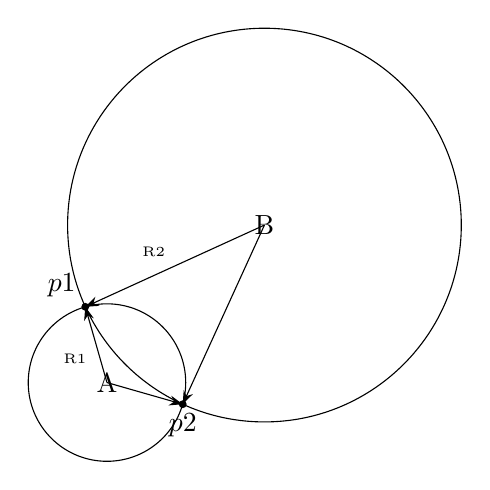
\begin{tikzpicture}[
cell label/.style = {text centered},
>=Stealth,
]

\coordinate (A) at (0,0);
\coordinate (B) at (2,2);

\node (C1) [name path=C1, draw, circle, minimum size=2cm] at (A){A};
\node (C2) [name path=C2, draw, circle, minimum size=5cm] at (B){B};


\path[name intersections={of=C1 and C2, by={[label=above left:$p1$]p1, [label=below:$p2$]p2}}];

\fill (p1) circle[radius=0.05cm];
\fill (p2) circle[radius=0.05cm];

\draw[->] (A) -- node[auto]{\tiny{R1}}(p1);
\draw[->] (A) -- (p2);
\draw[->] (B) -- node[auto,swap]{\tiny{R2}}(p1);
\draw[->] (B) -- (p2);

\end{tikzpicture}

\end{document}
